\section{预备知识}\label{preliminaries}

\subsection{神经辐射场(Nerual\; Radiance\; Field, NeRF)}

NeRF以一系列位姿已知的图片以及相机内参与外参作为输入,隐式的表达一个连续三维场景。如图\ref{nerf}所示,其使用了一个多层感知机(MLP)实现了以下映射:从一个连续的5D向量,
即空间坐标$\mathbf{x}=(x,y,z)$和视线方向$\mathbf{d}=( \theta,\varphi )$,到一个连续的3D场景密度$\sigma$ 和颜色$\mathbf{c}=(r,g,b)$。
该映射可以抽象为仅以3D坐标作为输入的函数$\sigma (\mathbf{x})$和同时以3D坐标与视线方向作为输入的函数$\mathbf{c(x,d)}$。

NeRF使用体渲染的方式,采用分层采样的方式进行积分,从而计算单个像素的颜色。
在一次计算中,给定一条从相机投影空间中心出的,穿过待计算像素的光线$\mathbf{r}(t)=\mathbf{o}+t\mathbf{d}$,
从其近边界遍历至其远边界($t_n$和$t_f$),并当中随机采样K个点$\{t_k\}_{k=1}^K$进行积分,得到的颜色如下:

\begin{equation}
    \hat{\mathbf{C}}(\mathbf{r})=\sum_{k=1}^{K}\hat{T}(t_k)\alpha(\sigma(t_k)\delta_k)\mathbf{c}(t_k)\;,
\end{equation}

\begin{equation}
     \mbox{其中} \quad \hat{T}(t_k)=\exp{\left (-\sum_{j = 1}^{k-1}\sigma(t_j)\delta_j\right )}\;,
\end{equation}

其中$\alpha(x)=1-\exp{(-x)}$, $\delta_k=t_{k+1}-t_k$为两个相邻采样点的距离。上述计算过程是可微的,因此给定一系列不同视角的图片, NeRF可以使用随机梯度下降法来优化$\sigma$和$\mathbf{c}$,从而最小化观察值与计算值的差异。与此同时, NeRF对输入使用位置编码来改善神经网络对高频信息的学习, 并且在物体表面附近增大采样率以提高采样效率。

\begin{figure}[htbp]
    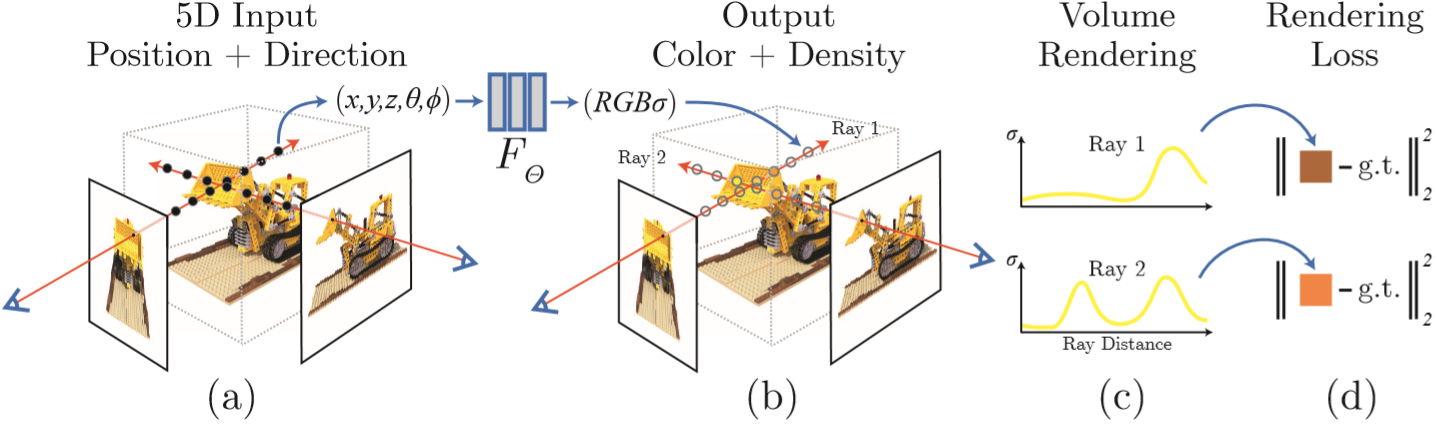
\includegraphics[scale = 1.2]{figures/nerf.png}
    \centering
    \caption{NeRF场景隐式表达与可微渲染过程,图源NeRF\cite{nerf}。沿着相机光线采样5D向量作为输入(a),通过MLP获得密度与颜色(b),最终通过体渲染的方式获得像素最终的颜色(c)。上述过程均可微,因此可以通过最小化观测值与计算值差距进行优化(d)。} \label{nerf}
\end{figure}
\subsection{符号距离场(Signed Distance Function, SDF)}
本文选择使用符号距离场函数\cite{sdf}来对场景的几何信息进行编码,而不使用体密度或占据概率。SDF是一种在空间中隐式表示表面的函数,其数学定义如下:

如果$\Omega$是以$d$为单位的度量空间$X$的子集,那么符号距离场函数$f$定义为:

$$f(x) = \left\{
\begin{aligned}
&d(x,\partial\Omega)&&if\; x\in\Omega \\
-&d(x,\partial\Omega)&&if\; x\notin\Omega\\
\end{aligned}
\right.
$$

$\partial\Omega$指$\Omega$的边界。对任意$x\in X$, $\inf$表示下确界,

$$
d(x,\partial\Omega) := \inf_{y\in \partial\Omega}d(x,y)
$$

简单的说,相较于显示的给定一个点与其法向量以表示一个表面,符号距离场函数映射了空间中一个点到某个表面的最近距离。如图如图\ref{sdf_figure}所示,值的符号取决于该位置位于平面的内部或外部。同时,为限制计算消耗与更精确的表示表面,本文为SDF设置了一个截断距离$tr$,即绝对值大于此值的SDF值被视为该值。
\begin{figure}[htbp]
    \centering
    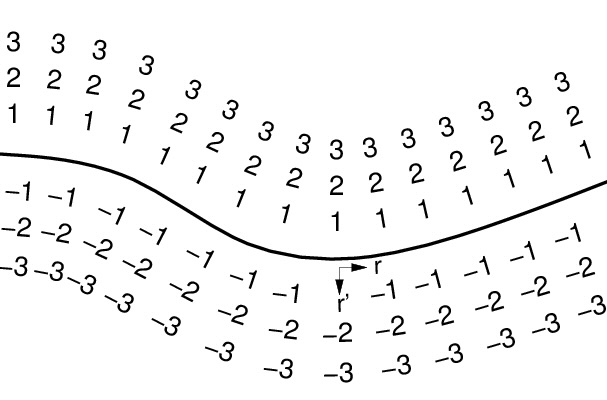
\includegraphics[scale=0.3]{figures/sdf_figure.jpeg}
    \caption{符号距离场函数}\label{sdf_figure}
\end{figure}
\subsection{八叉树(Octree)与空间莫顿码(Morton Code)}
\begin{figure}[htbp]
    \centering
    \subfigure{
    \begin{minipage}[t]{0.47\linewidth}
    \centering
    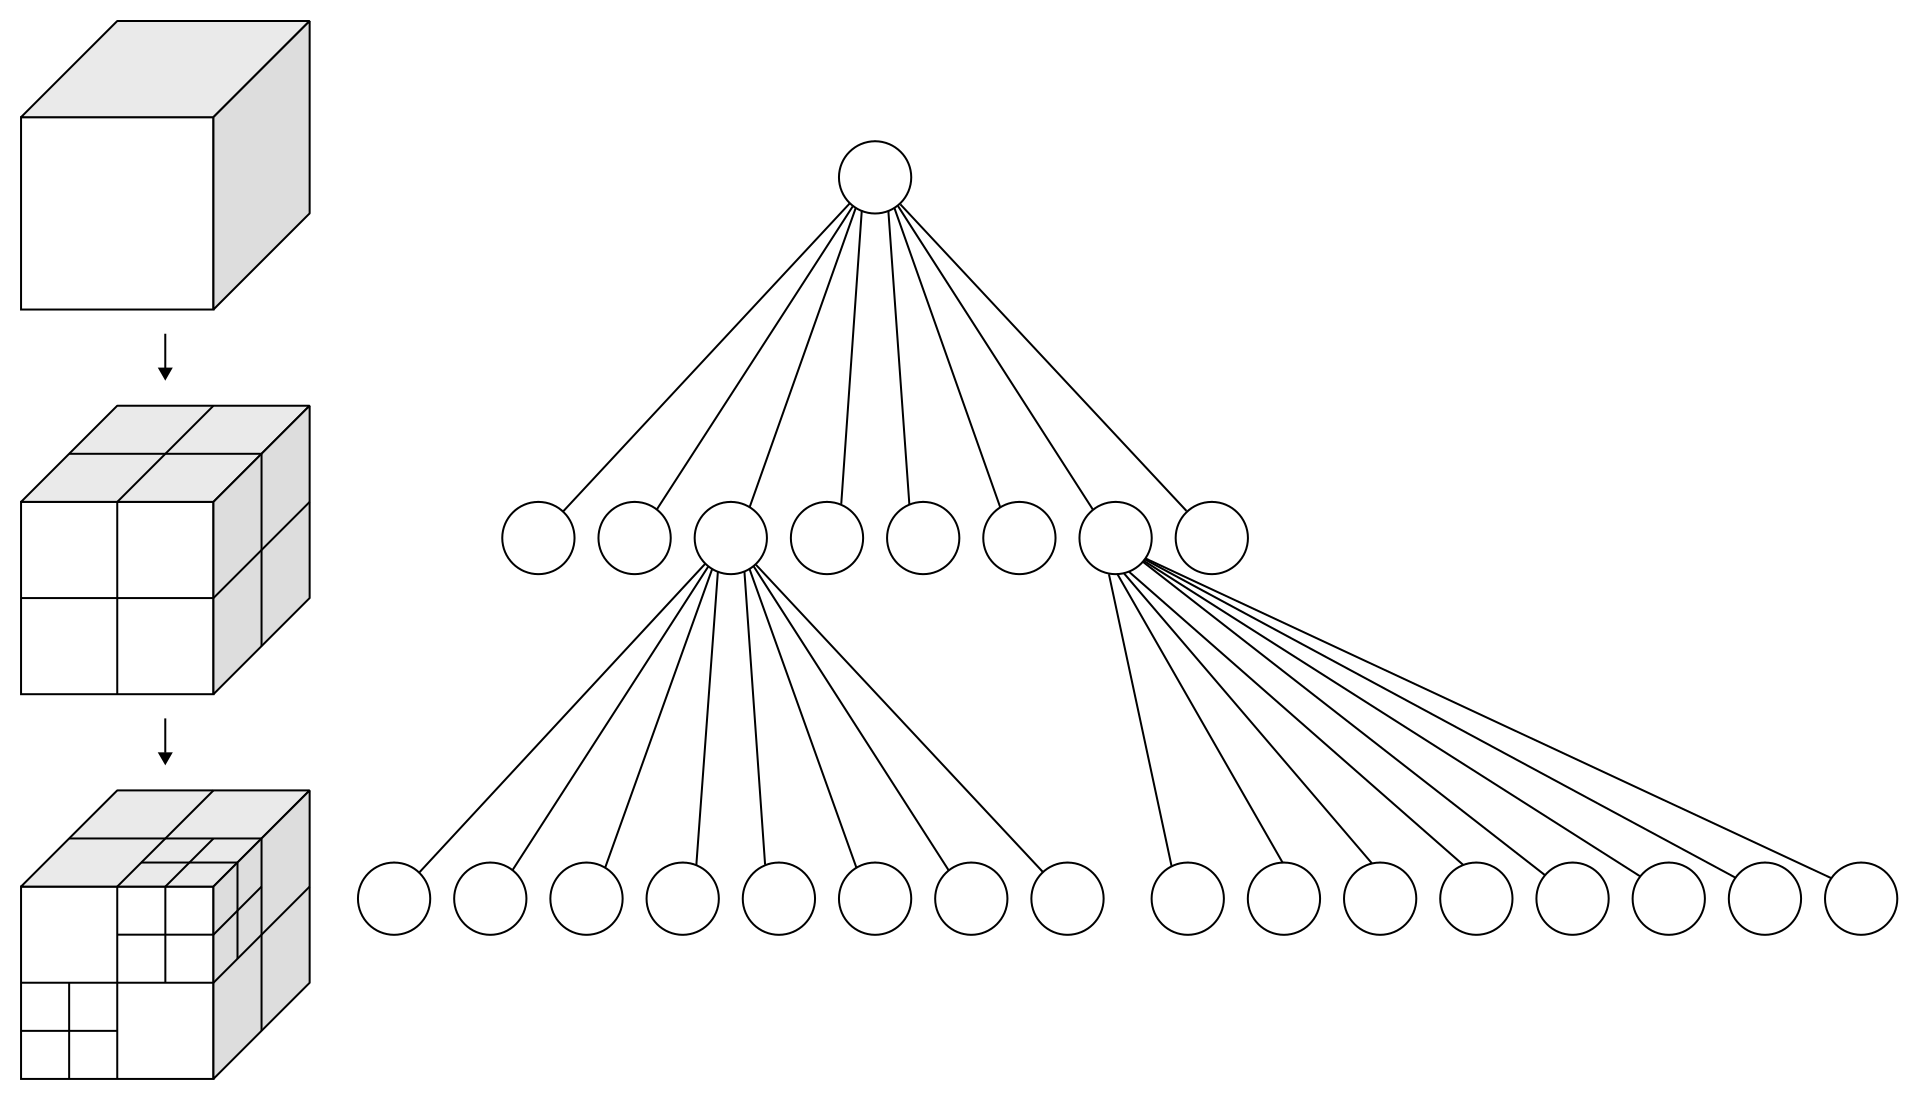
\includegraphics[width=\linewidth]{figures/octree.png}
    \caption{一个三层八叉树示例}\label{octree}
    \end{minipage}
    }
    \centering
    \subfigure{
    \begin{minipage}[t]{0.47\linewidth}
    \centering
    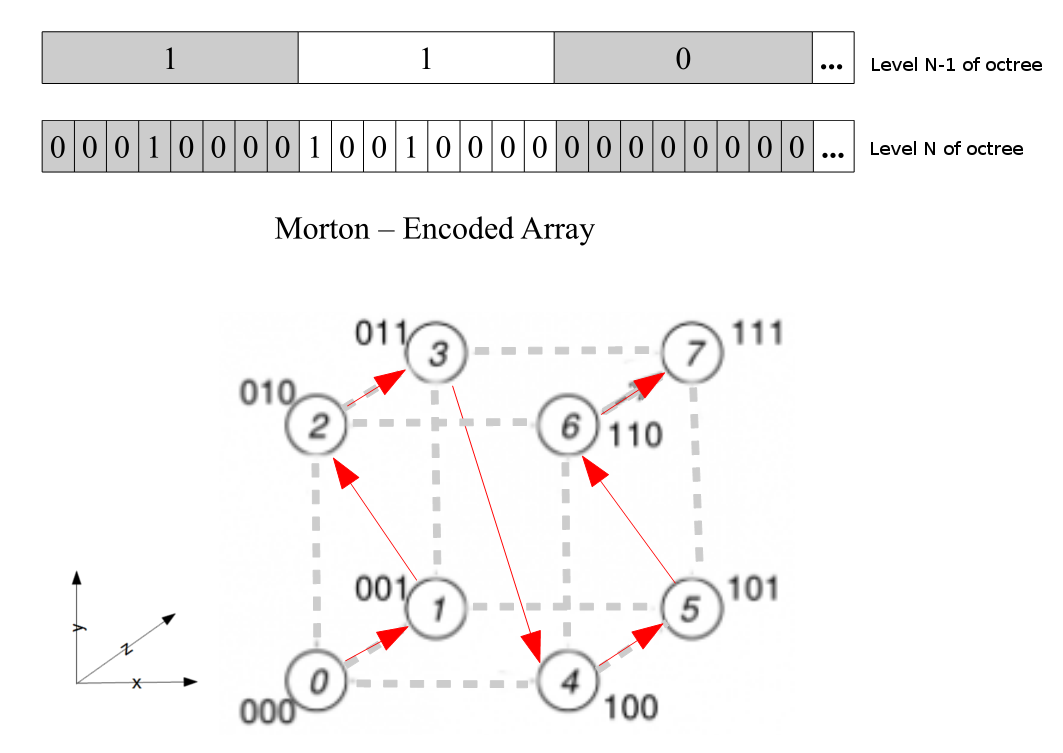
\includegraphics[width=\linewidth]{figures/morton.png}
    \caption{使用莫顿码将空间坐标编码至数组中}\label{morton}
    \end{minipage}
    }
\end{figure}
八叉树是一种用于描述三维空间的树状数据结构。如图\ref{octree},八叉树通过对三维空间的几何实体以循环递归的划分方法进行体元剖分,每个体元具有相同的时间和空间复杂度。在八叉树结构中如果被划分的体元具有相同的属性,则该体元构成一个叶节点;否则继续对该体元剖分成8个子立方体。使用八叉树可以快速进行三维目标的集合运算,如交、并、补、差等,也可快速进行临近点查询和与其他物体的碰撞检测。

为了快速的查询体素八叉树,本文使用了传统的基于体素的SLAM方法\cite{traditionalslam}中的方法,将体素坐标编码为莫顿码,并将体素中的信息线性存储,以此达到快速检索的目的。莫顿码是通过将坐标的二进制形式的每个维度的每个比特交叉重组的方式生成的,类似于一种哈希算法,将一个2D或3D坐标转换为一个唯一的索引。如图\ref{morton}所示,给定一个体素的3D坐标$(x,y,z)$,通过遍历其莫顿码,本文可以快速的找到其在八叉树中的位置。同时,本文也可以对当前体素的莫顿码进行变换以快速找到其相邻的体素。
